% a{More Analysis}nofficial University of Oxford Poster Template
% https://github.com/andiac/gemini-cam
% a fork of https://github.com/anishathalye/gemini

\documentclass[final]{beamer}

% ====================
% Packages
% ====================

\usepackage[T1]{fontenc}
\usepackage{lmodern}
\usepackage{lipsum}
\usepackage[size=custom,width=84,height=59,scale=1.0]{beamerposter}

\usetheme{gemini}
\usecolortheme{NOAA}
\usepackage{graphicx}
\usepackage{booktabs}
\usepackage{tikz}
\usepackage{pgfplots}
\pgfplotsset{compat=1.14}
\usepackage{anyfontsize}
\usepackage{wrapfig}
\usepackage{subcaption}
\usepackage[font=footnotesize,skip=10pt]{caption} %default 30pt

\usepackage[style=numeric, sorting=none, isbn=false, url=false]{biblatex}
\addbibresource{refs.bib}



% ====================
% Lengths
% ====================

% If you have N columns, choose \sepwidth and \colwidth such that
% (N+1)*\sepwidth + N*\colwidth = \paperwidth
\newlength{\sepwidth}
\newlength{\colwidth}
\setlength{\sepwidth}{0.025\paperwidth}
\setlength{\colwidth}{0.3\paperwidth}

\newcommand{\separatorcolumn}{\begin{column}{\sepwidth}\end{column}}
\renewcommand*{\bibfont}{\normalfont\tiny}

% ====================
% Title
% ====================

\title{Subregional Analysis of Great Lakes Ice Cover: \\  Connecting Ice to Local Weather Data}

\author{James Kessler \inst{1} \and David Cannon \inst{2} \and Alisa Young \inst{1} \and Jia Wang \inst{1}}

\institute[shortinst]{\inst{1} NOAA Great Lakes Environmental Research Lab \samelineand \inst{2} Cooperative Institute for Great Lakes Research}

% ====================
% Footer (optional)
% ====================

\footercontent{
\href{http://www.glerl.noaa.gov}{www.GLERL.NOAA.gov} \hfill
  Ocean Science Meeting 2026, Glasgow, Scotland, U.K.  \hfill
\href{mailto:james.kessler@noaa.gov?subject=OSM Poster}{james.kessler@noaa.gov}}
% (can be left out to remove footer)

% ====================
% Logo (optional)
% ====================
% Refer to https://github.com/k4rtik/uchicago-poster
% logo: https://communications.admin.ox.ac.uk/communications-resources/visual-identity/identity-guidelines/the-oxford-logo
% use this to include logos on the left and/or right side of the header:
\logoright{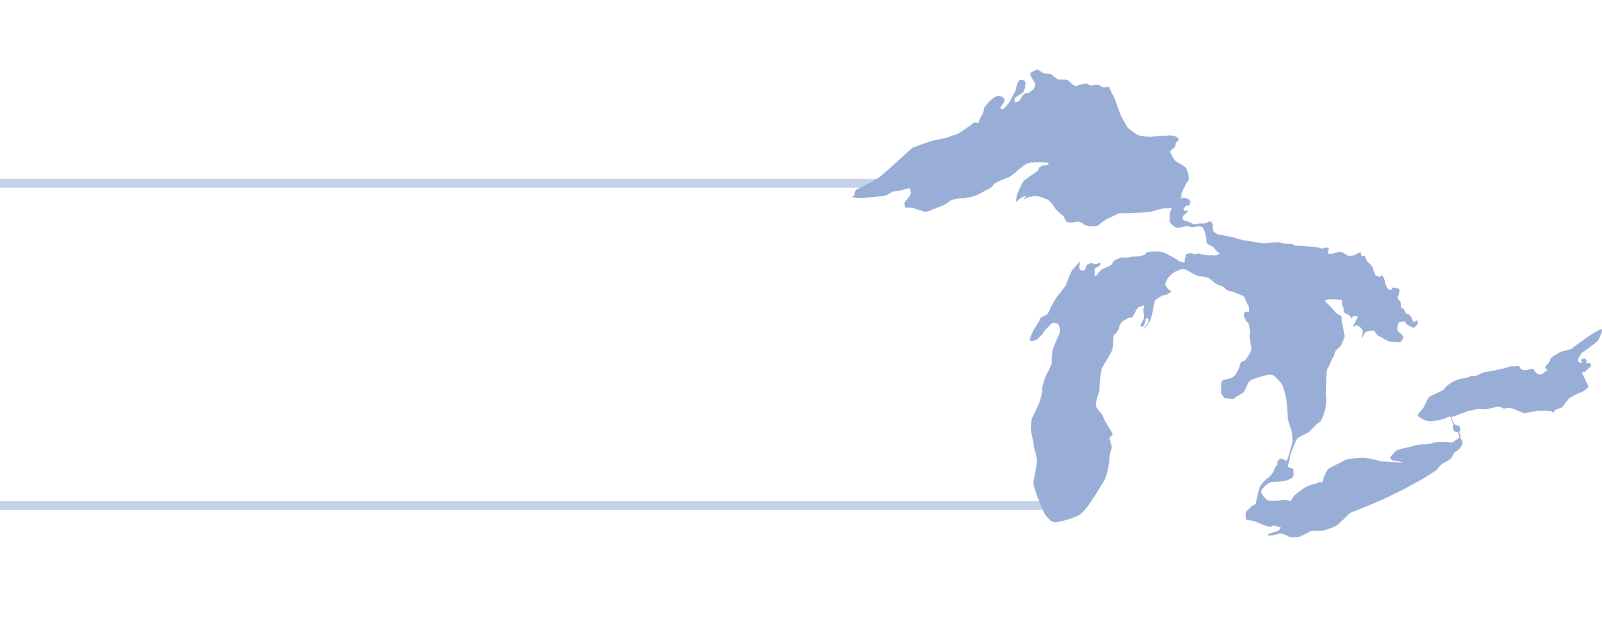
\includegraphics[height=3cm]{logos/CIGLR_LOGO_white.png}}
\logoleft{
\includegraphics[height=3cm]{logos/GLERL.png}}

% ====================
% Body
% ====================

\begin{document}

	\small
\begin{frame}[t]
\begin{columns}[t]
\separatorcolumn
\begin{column}{\colwidth}

	\begin{block}{Introduction} \label{intro}
		Ice cover in the Great Lakes  highly variable and has significant influence on regional climate, ecology, and economy. Spatially resolved ice cover ($\Delta x=1.25 \textup{KM}^2$) has been recorded since 1973 and is available as daily files throughout each ice season\supercite{Yang2020}. Previous work has assessed large-scale (i.e. lake or basin-wide) ice cover fluctuations through time and their relationship to global weather phenomena \supercite{Mason2016, Sharma2019, OReilly2015, Wang2018, Bai2012}. Following Mason et al. (2016)\supercite{Mason2016} we use the Great Lakes Aquatic Habitat Framework (GLAHF)\supercite{Wang2015} to analyze ice cover on a subregional basis for the below metrics and analyze how morphometry (area, depth, etc.) and atmospheric conditions impact ice cover in the Great Lakes.
	\begin{itemize}
		  \item \textbf{Annual Max Ice Cover (AMIC):} maximum percent during a given season
		  \item \textbf{Seasonal Average Ice Cover (JFM):} mean daily ice cover:  Jan 1 - Mar 31
		  \item \textbf{Ice Duration:} Total (non-consecutive) days where ice cover exceeded 10\%
		\end{itemize}
  \end{block}

  \begin{block}{Methods} \label{methods}
    \begin{figure}
			  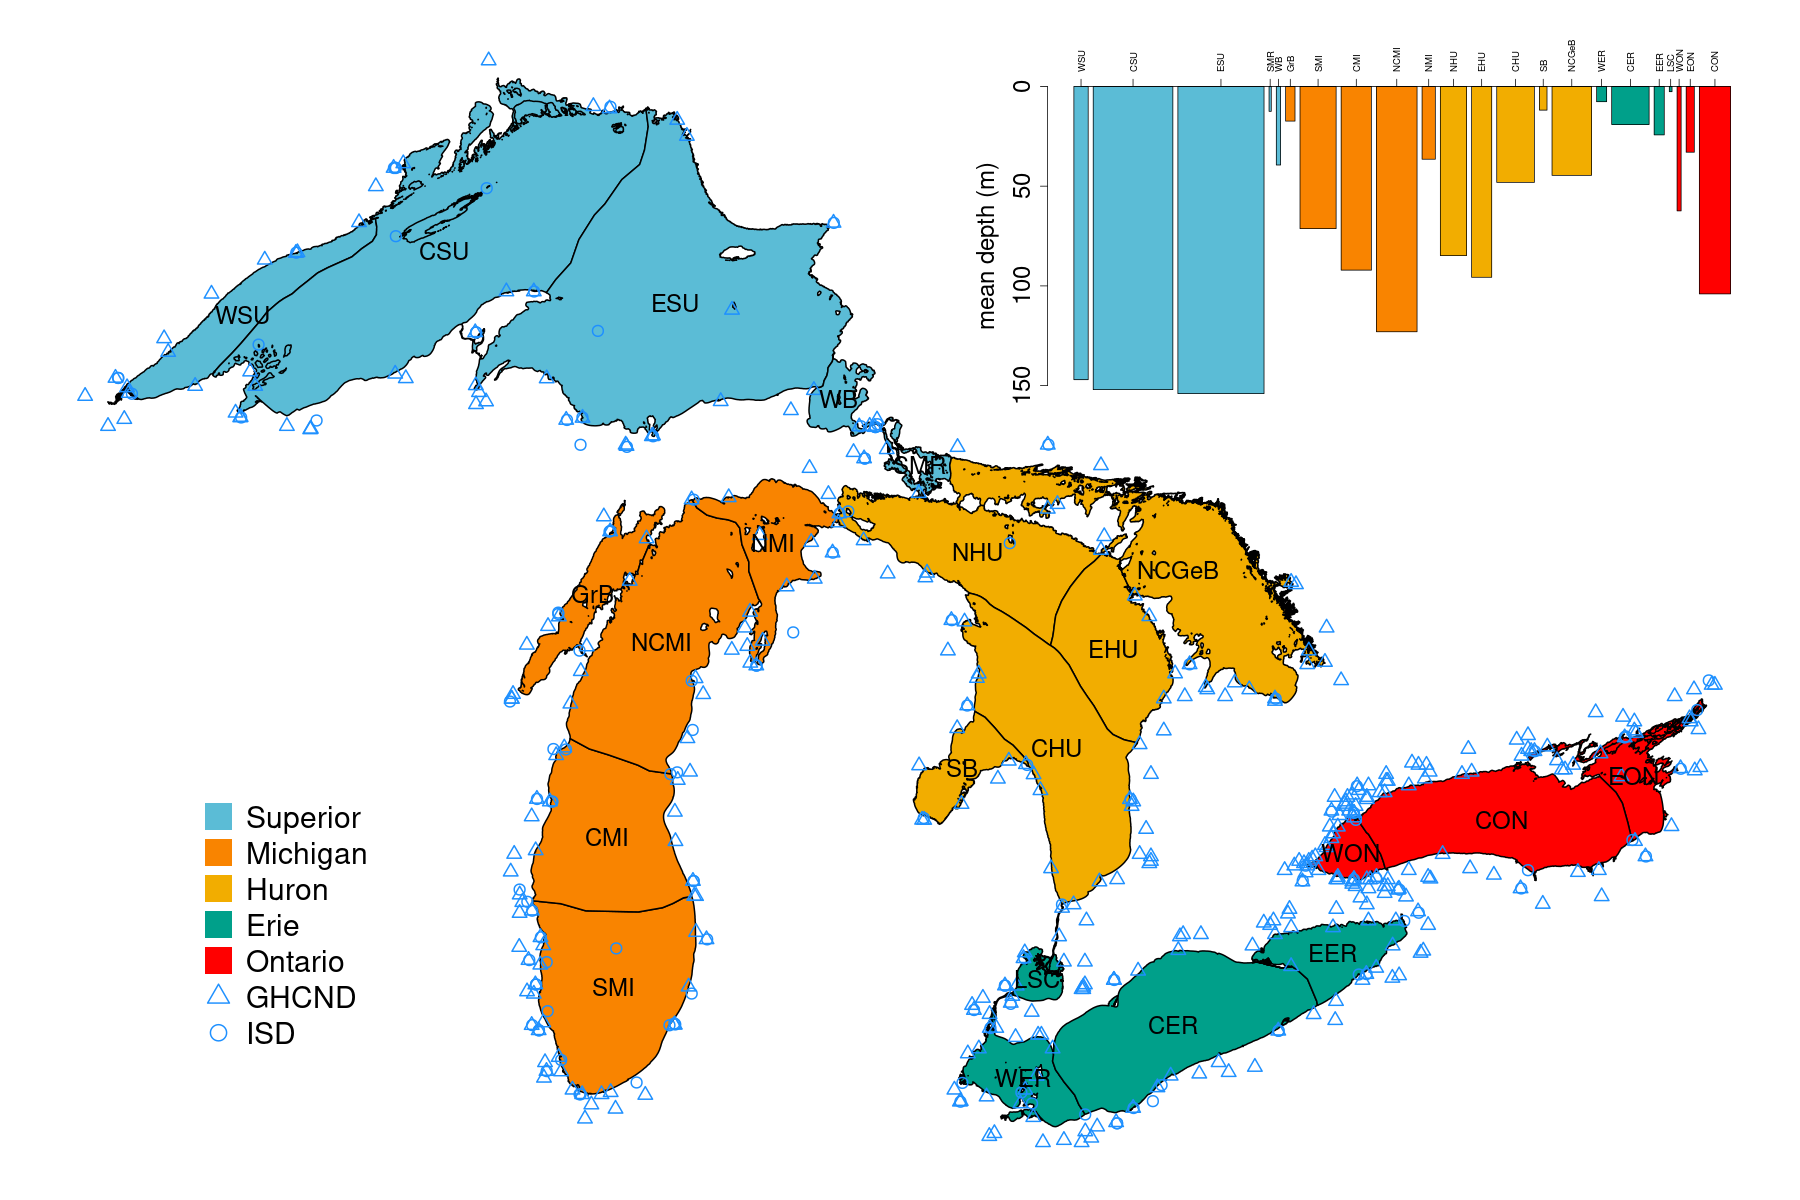
\includegraphics[width=.9\textwidth]{../figures/station_map.png}
			  \caption{Spatial delineation of GLAHF subregions and selected met station locations (GHCND\supercite{Menne2012}, ISD\supercite{Smith2011}). The upper right figure shows depth and (relative) surface area of each subregion in the y and x directions, respectively.}
			   \label{fig:map} 
	\end{figure}
	\vspace{-4ex}
	  \begin{enumerate}
	  \normalsize \bfseries
		  \item{Do ice trends exist at these spatial scales and how are they related to lake morphometry?}
		  \item{How do atmospheric conditions impact ice formation?}
 	 \end{enumerate}
	\justifying
	Q1: Ice metrics calculated for each subregion and Mann-Kendall monotonic trend test\supercite{Mann1945} performed; correlations between trend magnitude and morphometrics. \\
	\bigskip
	Q2: station data\supercite{Menne2012,Smith2011} aggregated for subregions based on a 20 KM radius; correlations identified between ice metrics and monthly mean (or max) meteorological conditions.



  \end{block}

\end{column}


\separatorcolumn
\begin{column}{\colwidth}
	\small
	\begin{block}{Analysis}\label{analysis}
\begin{figure} 
	 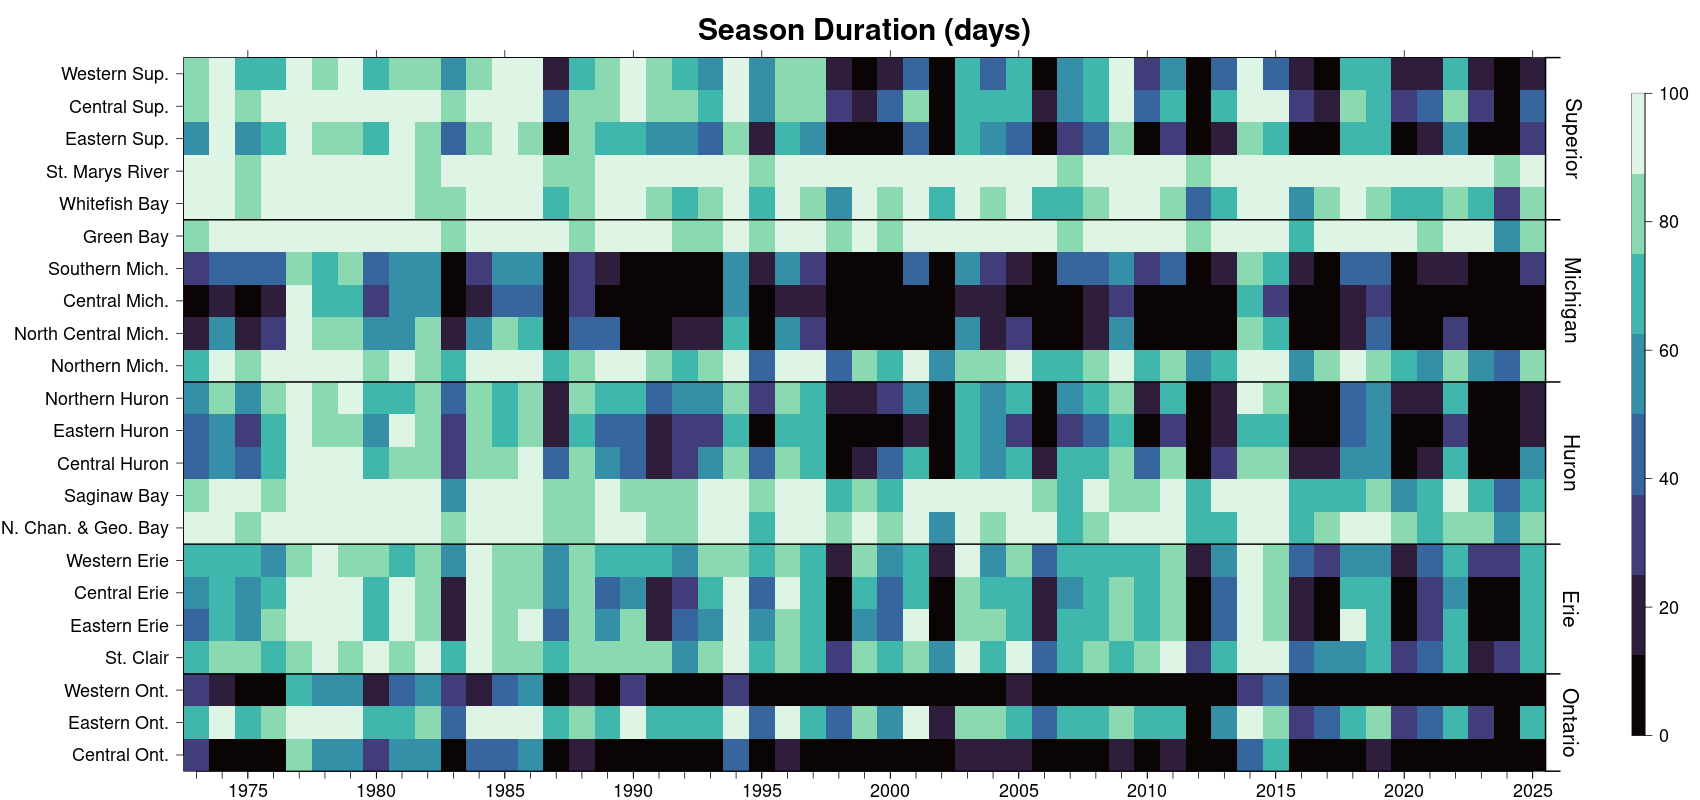
\includegraphics[width=.9\textwidth]{../figures/dur_ts.png} 
	 \caption{Evolution of one of three metrics analyzed (ice duration) for each subregion.}
	 \label{fig:dur}
\end{figure}
	\vspace{-5ex}
\begin{figure}
 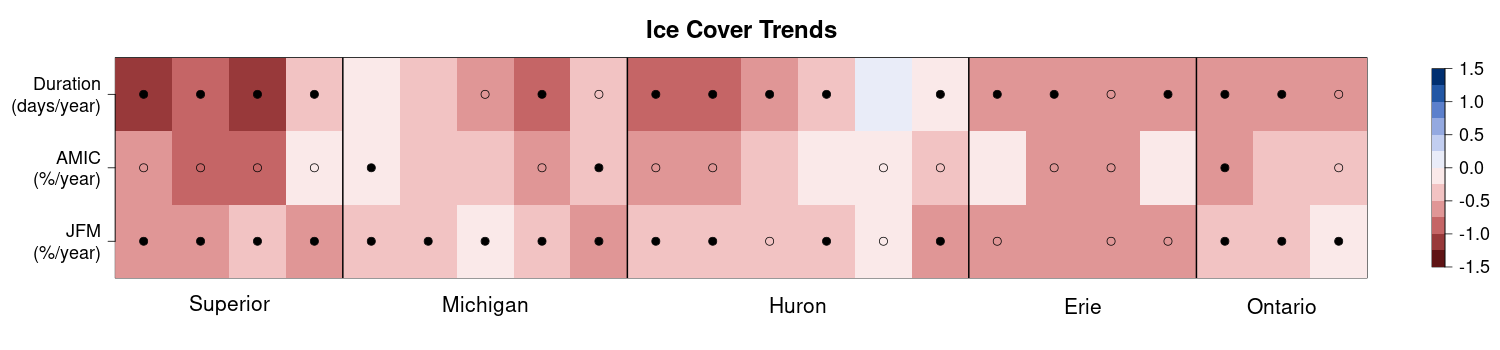
\includegraphics[width=\textwidth]{../figures/trends_horz.png} 
 \caption{Linear trends for each metric. Open (solid) dots indicate 95\% (99\%) statistical significance. Columns correspond to rows in fig \ref{fig:dur}. }
  \label{fig:trends}
\end{figure}
			Season duration decrease is visible in some (primarily deep) regions but not apparent in others (see fig. \ref{fig:dur}). This may be due to warmer subsurface temps\supercite{Cannon2024, Anderson2021} providing heat to surface waters and preventing freezing, whereas shallow regions are more frequently isothermal and thus able to release all heat from the water column. 
	\vspace{-2ex}
\begin{figure} 
	  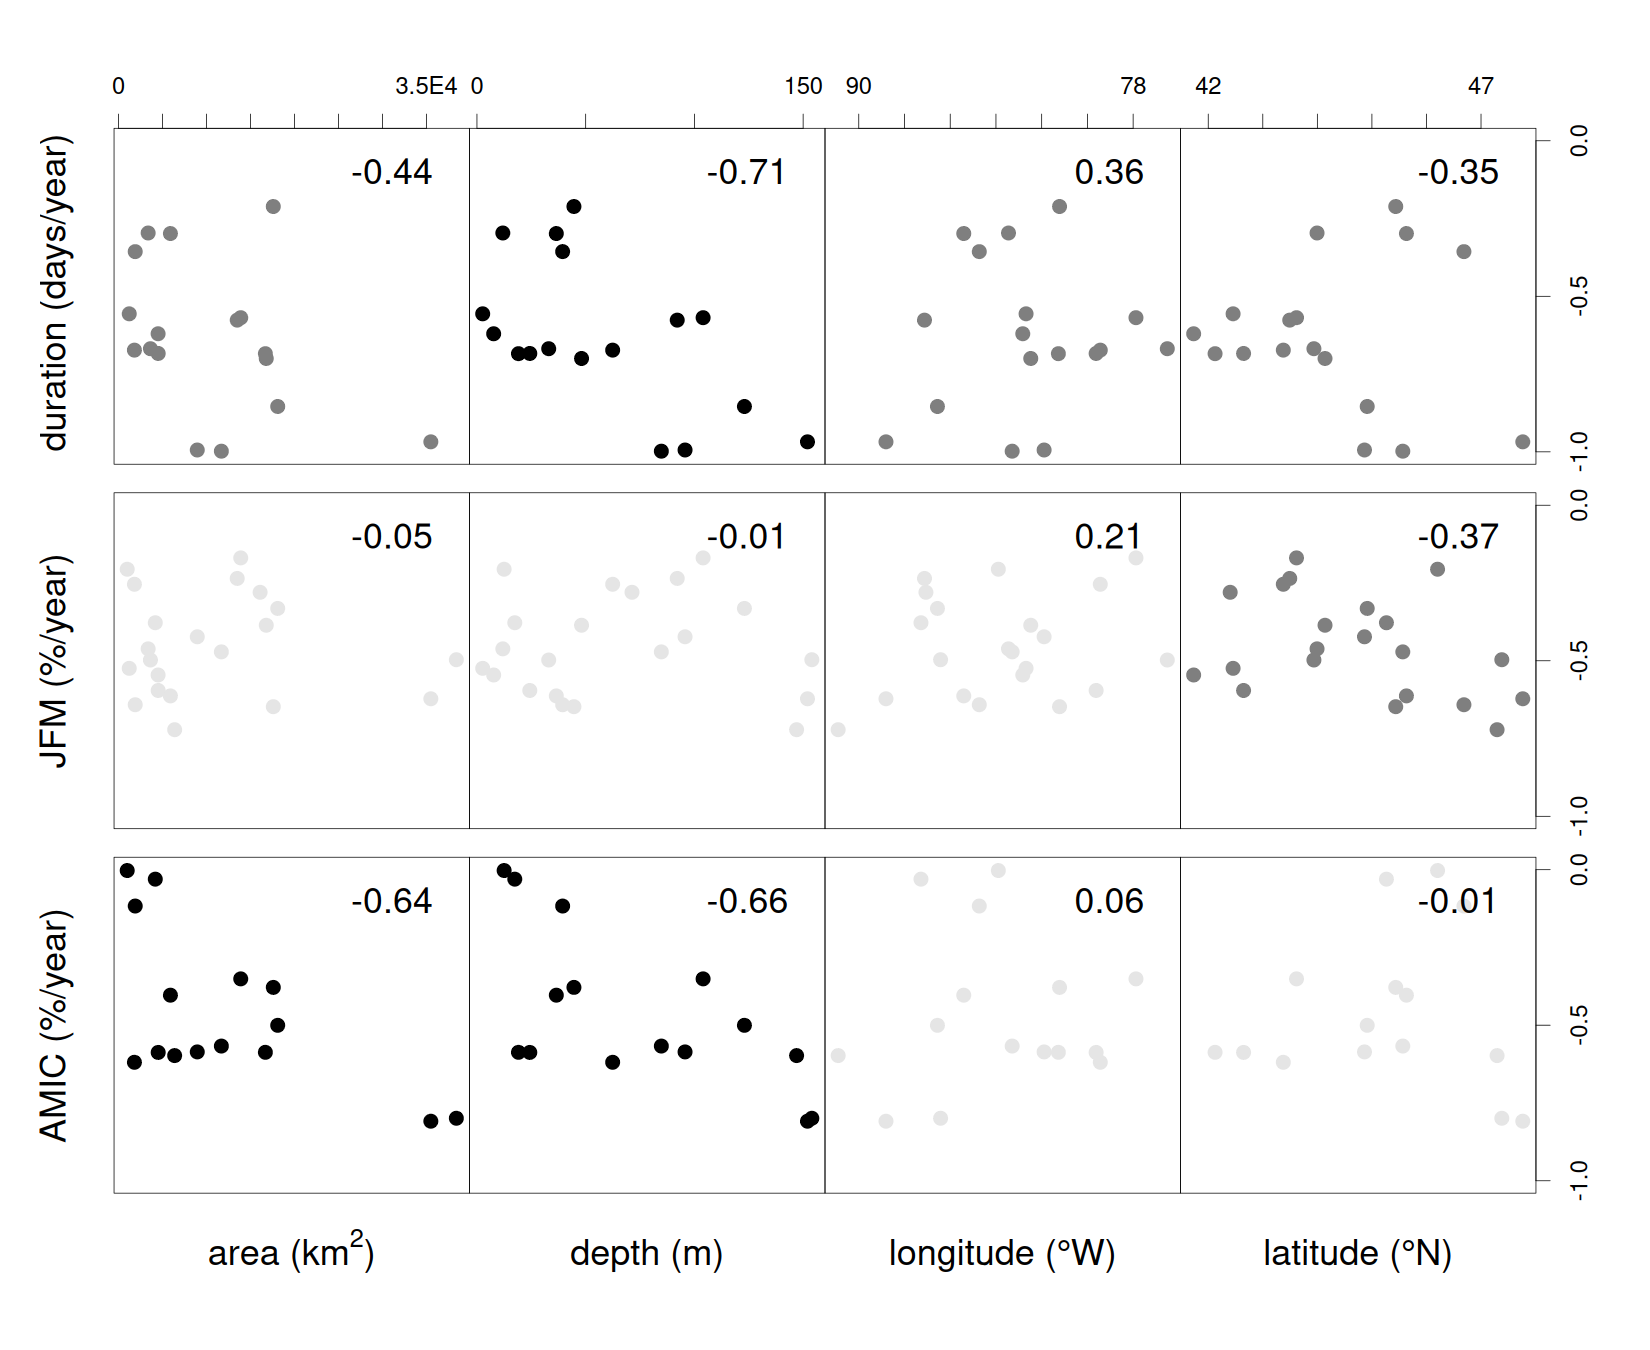
\includegraphics[width=0.7\textwidth]{../figures/morphoscatter.png}
	  \caption{Correlations between statistically significant ice metric trends (vertical axes) and morphometrics (horizontal axes). Moderate correlations (Pearson's r$>$0.3) are shown in dark grey and strong correlations ($>$0.6) are black.}
		\label{fig:boxplot}
\end{figure}
	\vspace{-3ex}

  \end{block}
\end{column}

\separatorcolumn

\begin{column}{\colwidth}

%	\centering	\large \textbf{\underline{Part 2: Correlation with Met Stations}} \normalfont
				Area (and depth) has significant influence on AMIC (and ice duration). Area's influence is curious, with larger surface areas providing more heat exchange at the surface. It should be noted that area, depth and volume (not shown), covary. Higher latitude regions showed more decrease in JFM and ice duration but not in AMIC.

	
	\begin{figure} 
		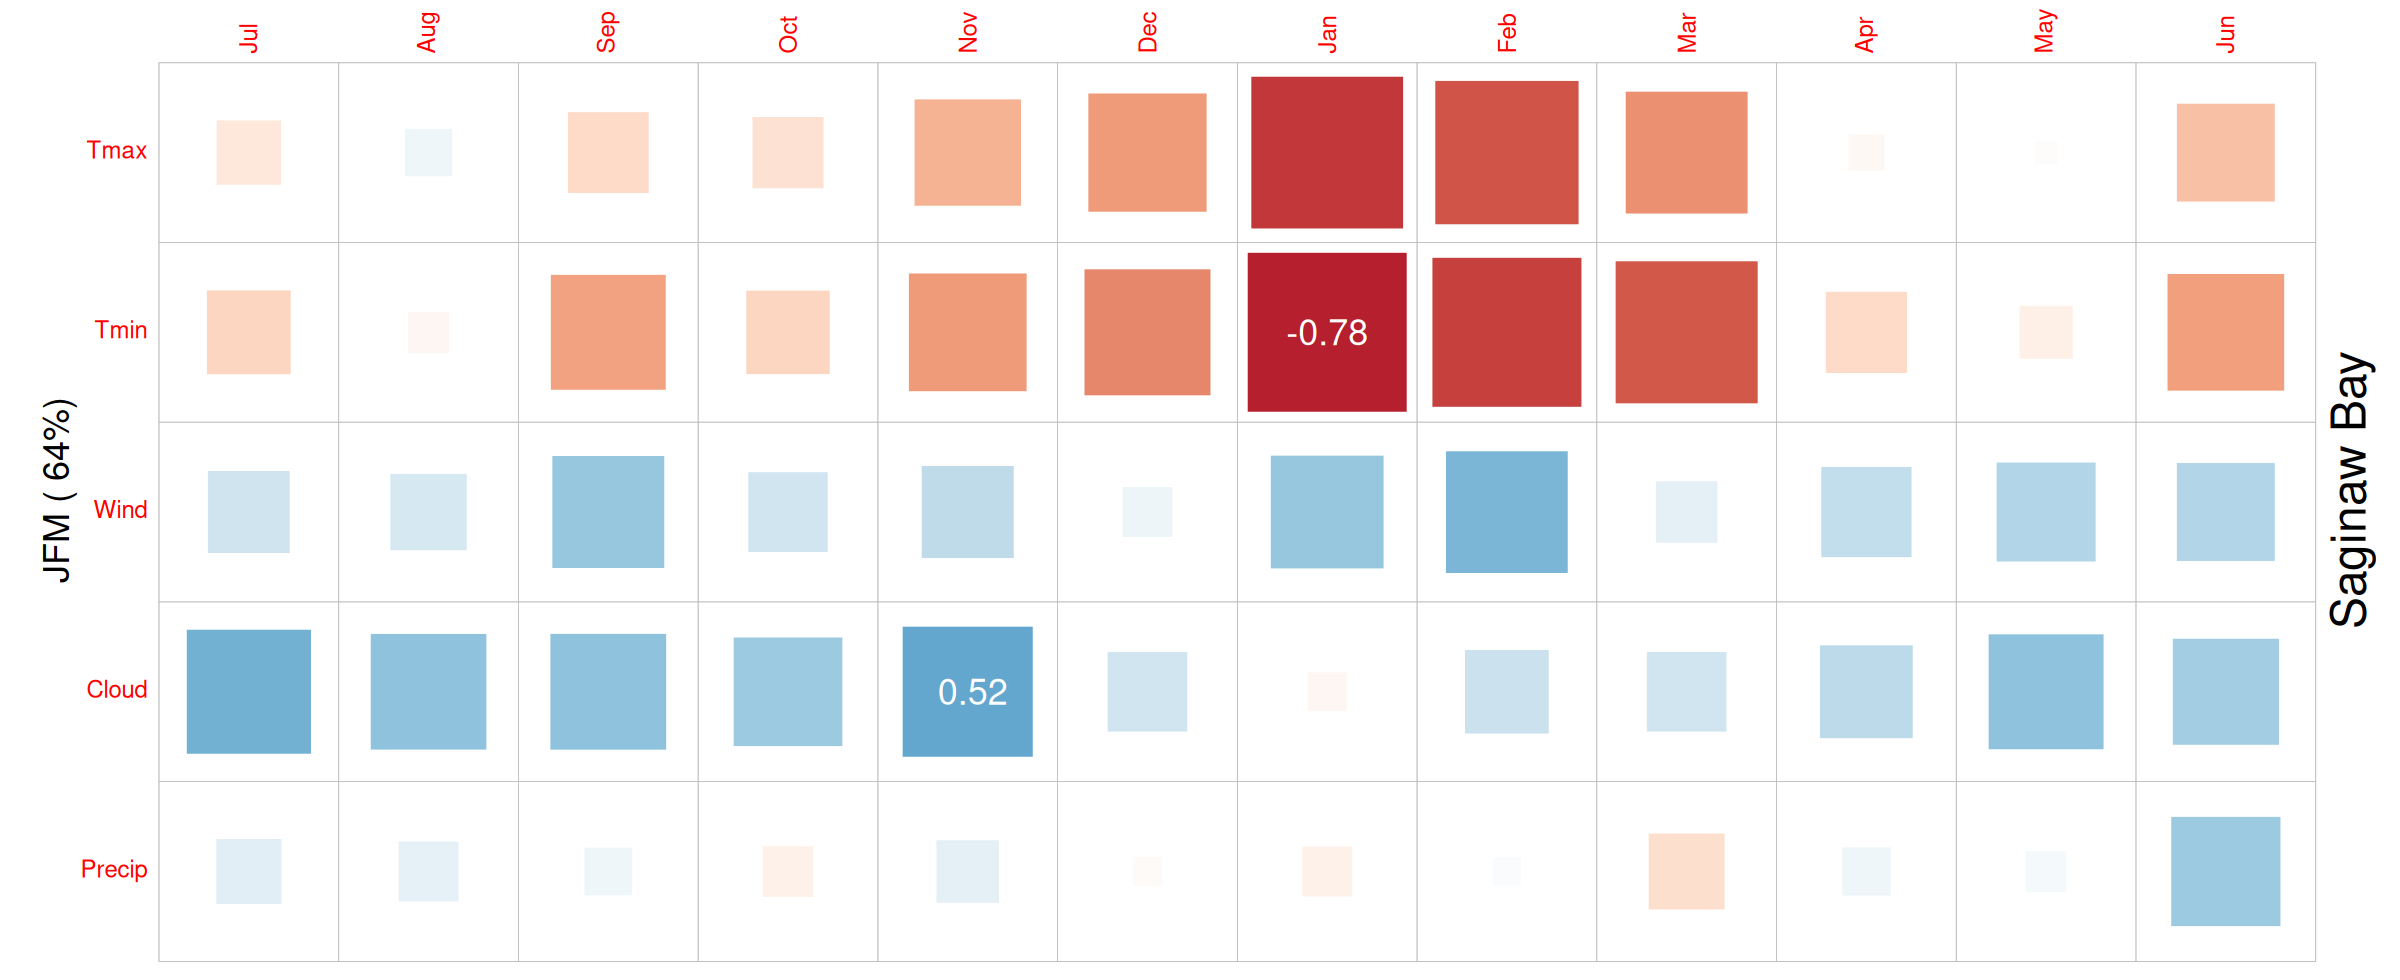
\includegraphics[width=0.9\textwidth]{../figures/cor/SB.png}
		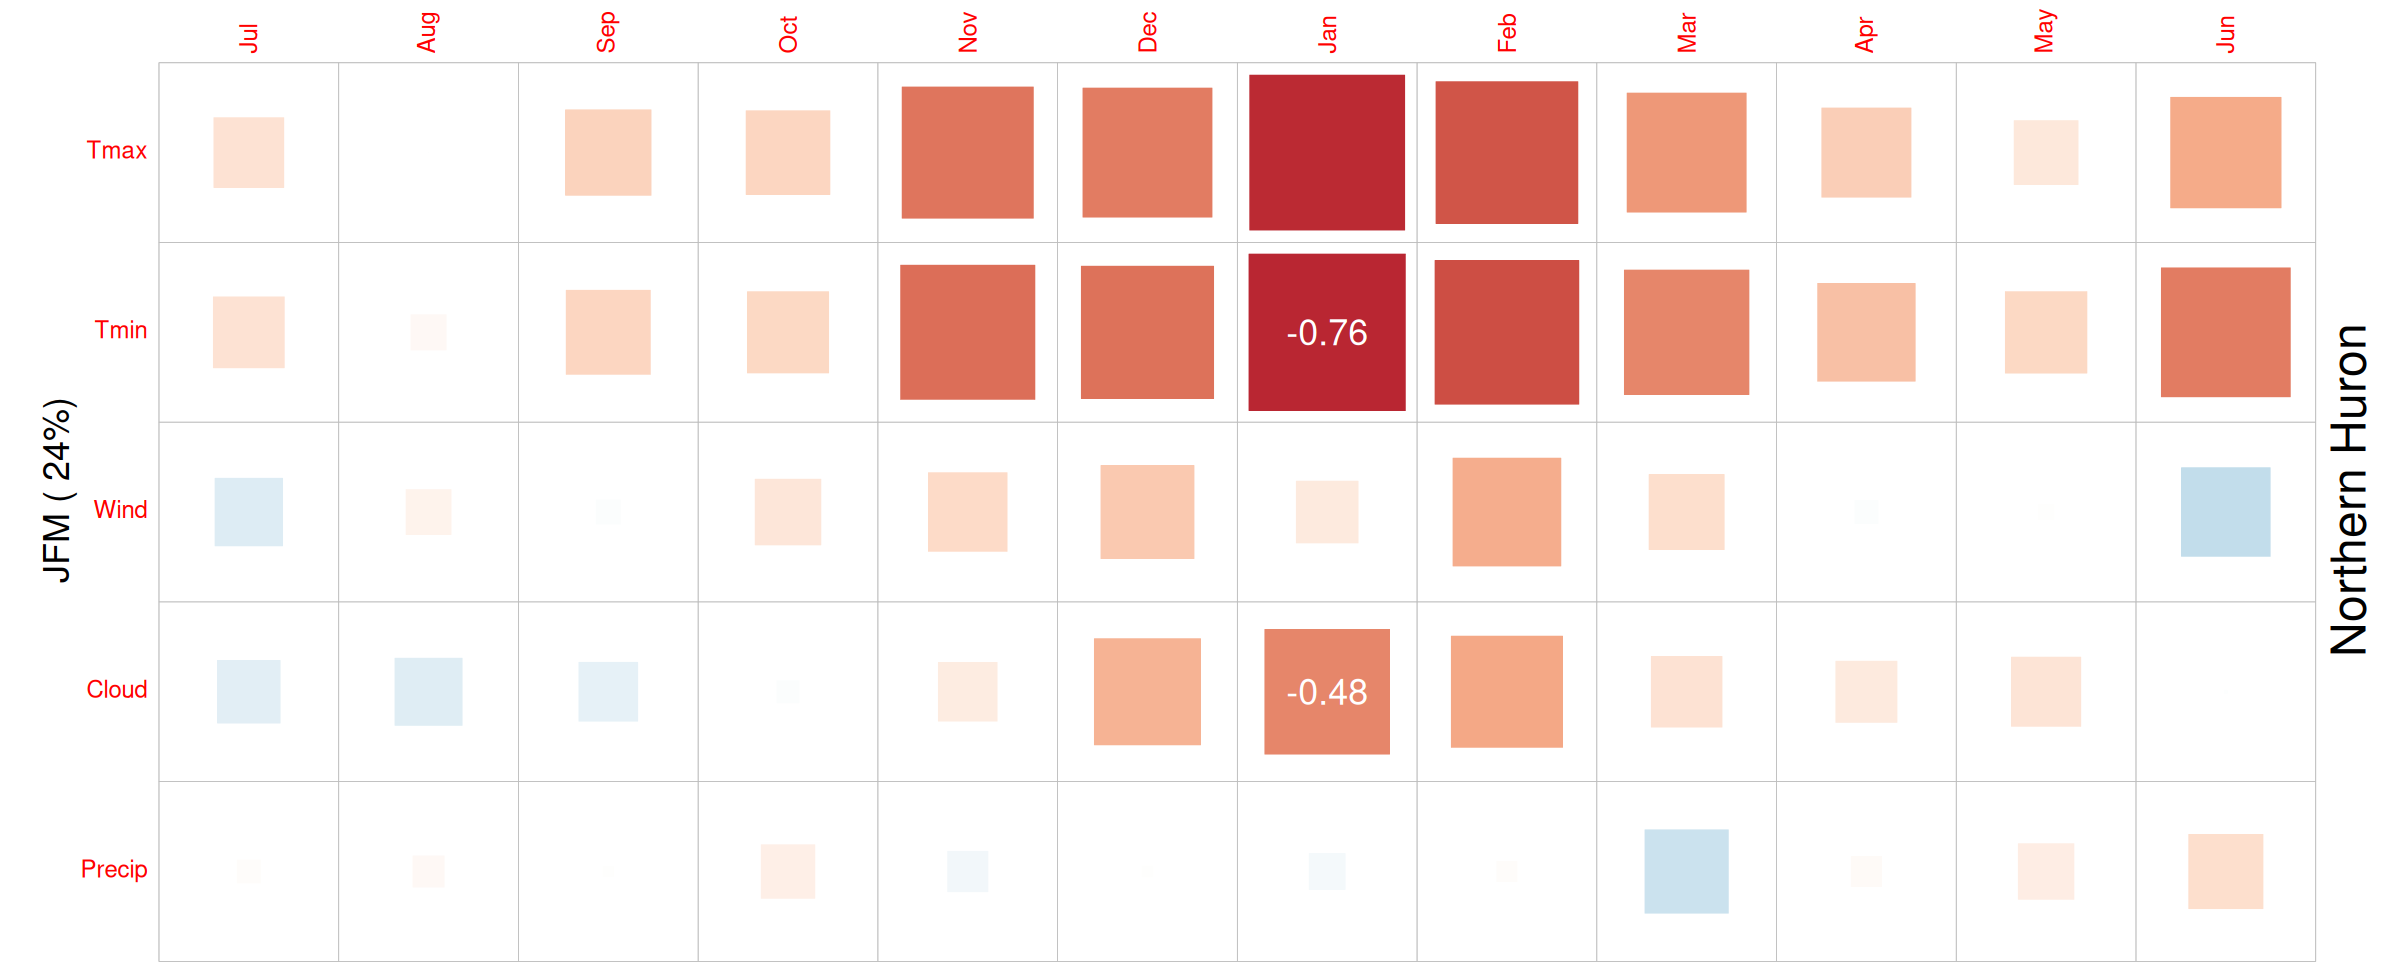
\includegraphics[width=0.9\textwidth]{../figures/cor/NHU.png}
		%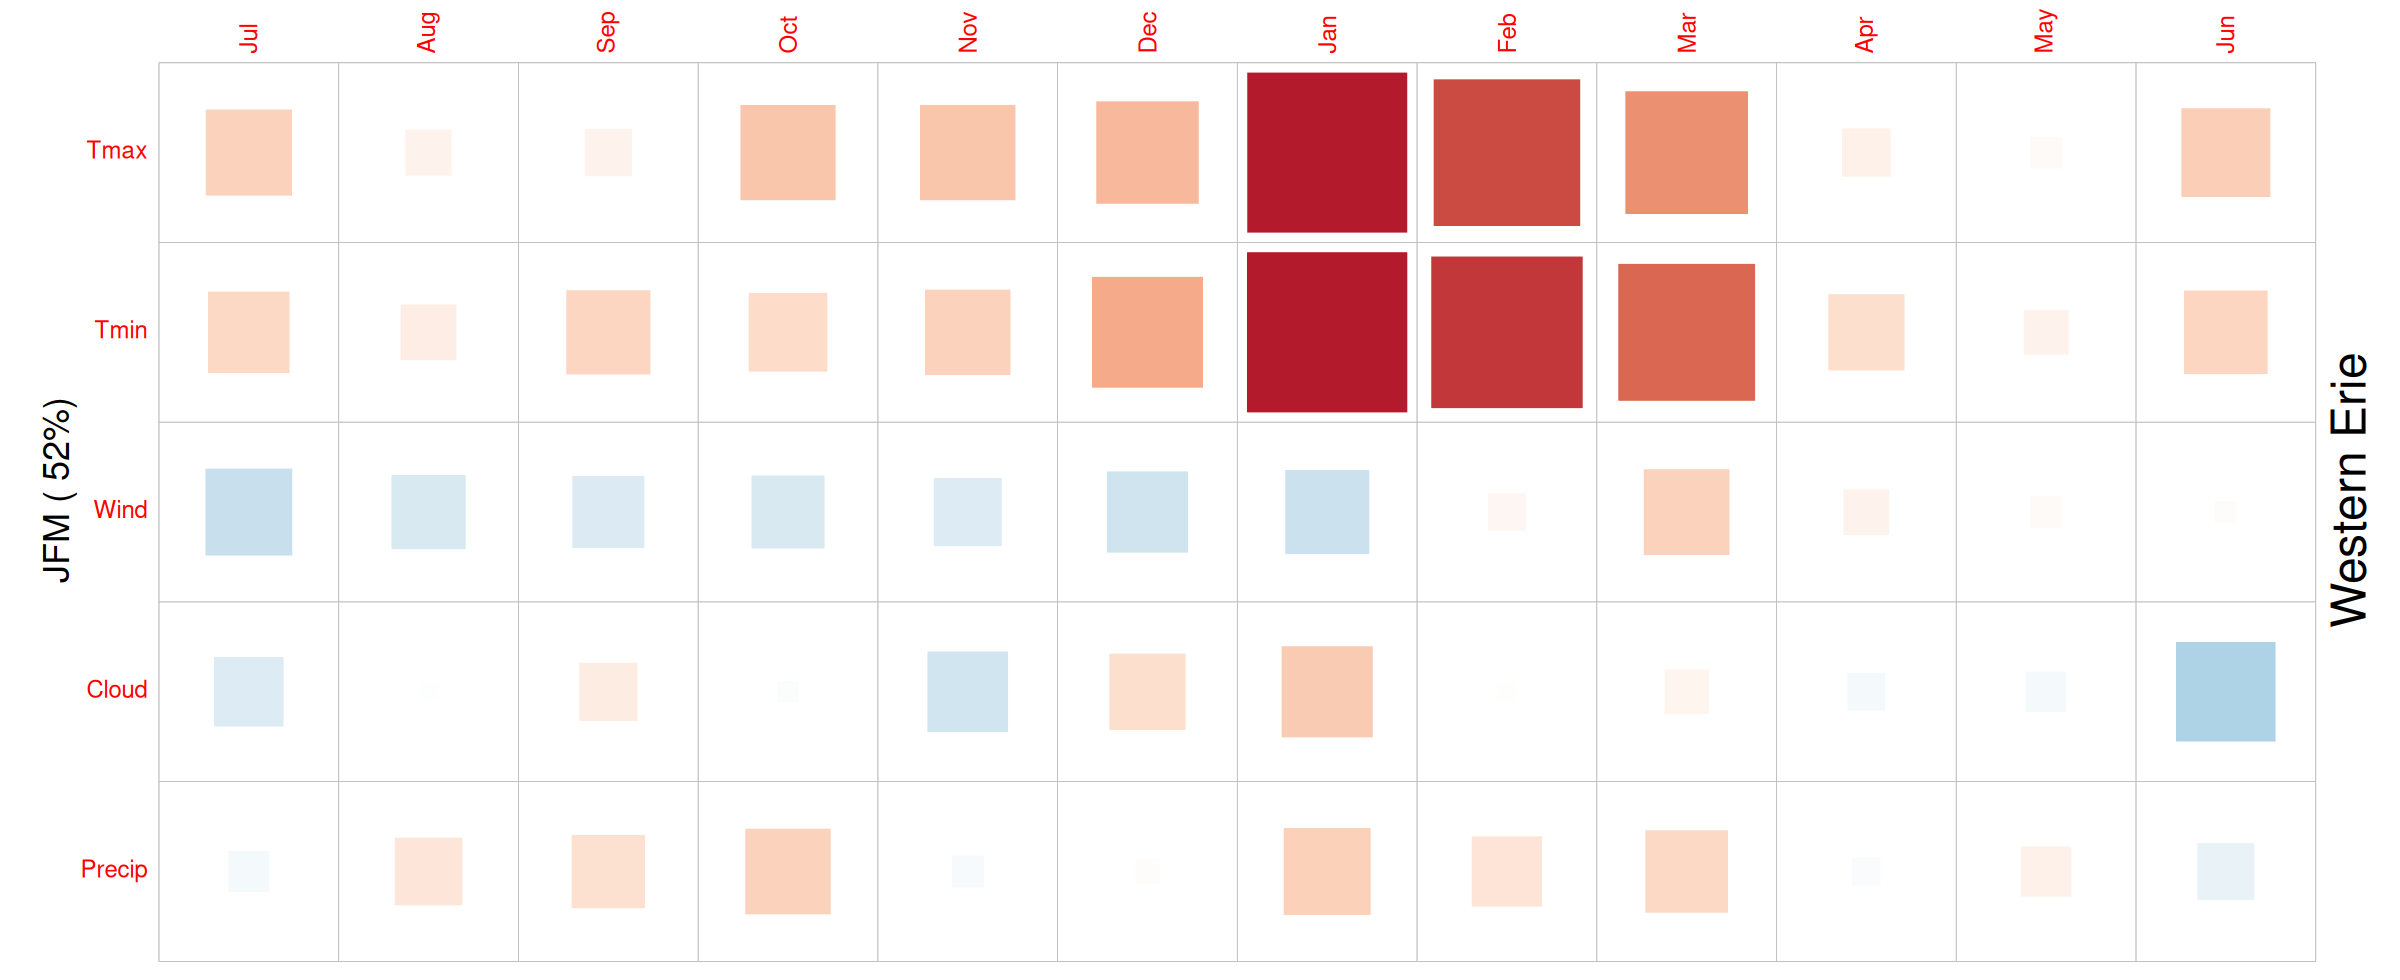
\includegraphics[width=\textwidth]{../figures/cor/WER.png}
		\caption{Correlation between Seasonal Ice Cover (JFM) and local meteorology. Meteorological variables are aggregated by month (columns) and state variable (rows). Data was correlated from Jul-Jun to each ice season during that window. Larger squares indicate stronger correlations and blue (red) indicates direct (indirect) correlation.}
	  \label{fig:scatter}
	  \end{figure}

	  \justifying

		  Strong inverse correlation was observed with air temp, particularly during Jan and Feb. Precip showed minimal correlation during any month/region while wind and cloud cover had moderate correlations. Since wind contributes to surface mixing which ultimately cools the water column during fall and clouds primarily reflect solar radiation, we expect direct correlations with ice cover (this was true for Saginaw Bay but not Northern Huron.) A number of post ice season correlations were identified--this provides valuable insight into physical processes but are not useful for prediction. 
		  \vspace{4ex}
\begin{block}{Summary}\label{summary}
		\begin{itemize}
			\item A majority of subregions show significant decreasing trends in all three metrics
			\item Lake morphology influences ice trends; not consistent across ice metrics
			\item Air temperature strongly anti-correlated with ice cover for all metrics
			\item Wind, cloud correlations with ice cover varied among subregions
			\item Future work: predictive model development: step-wise linear \\ regression or machine-learning
		\end{itemize}
		\vspace{-9ex}
		\raggedleft
		References: 
\includegraphics[width=.125\textwidth]{../figures/bib_qr.png}
  \end{block}

\end{column}

\separatorcolumn

\end{columns}

\end{frame}

\end{document}


